\lab{Algorithms}{B\'{e}zier Curves}{B\'{e}zier Curves}

\objective{Understand the basics of B\'{e}zier Curves and De Casteljau's algorithm}

There are many different ways of approximating functions. 
In computer graphics, spline curves are often used. 

One specific problem that any sort of approximation to a set of points must overcome is that it must be coordinate independent. 
This means that by rotating the coordinate axes, we do not actually change the curve. 
This is a problem with normal curve interpolation methods. 
The following is an example of two interpolating curves through a set of points in different coordinate systems.

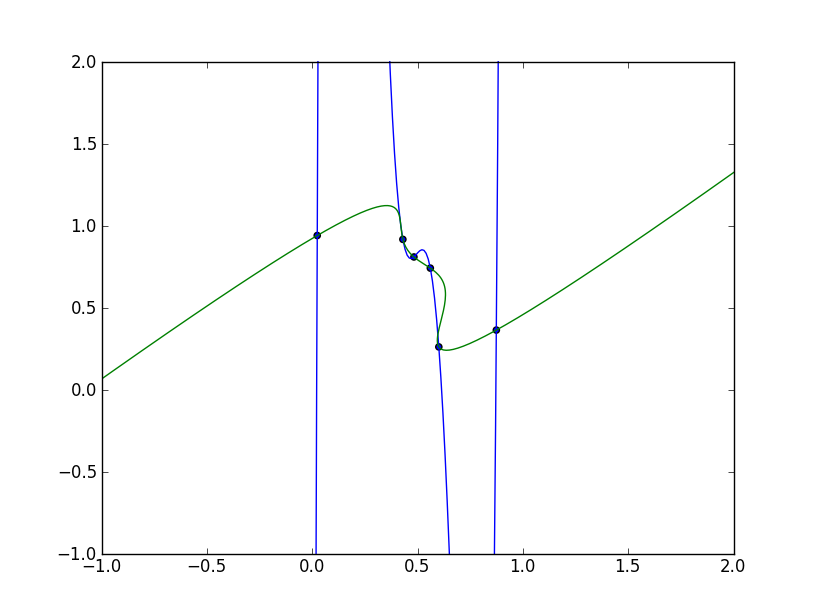
\includegraphics[width=\textwidth]{bad_interpolation}

Another problem with traditional interpolation is that, though the curve may pass through each point, its behavior between the points we are interpolating may be unpredictable, as in the following example. 
This is called Runge's Phenomenon. 
When doing approximation of a function, this can be abated by using carefully chosen interpolation points; however, when we are trying to approximate a given set of points we will probably not be able to choose exactly what we are given. 
Carefully choosing interpolation points still leaves us with the rotation problem illustrated above.

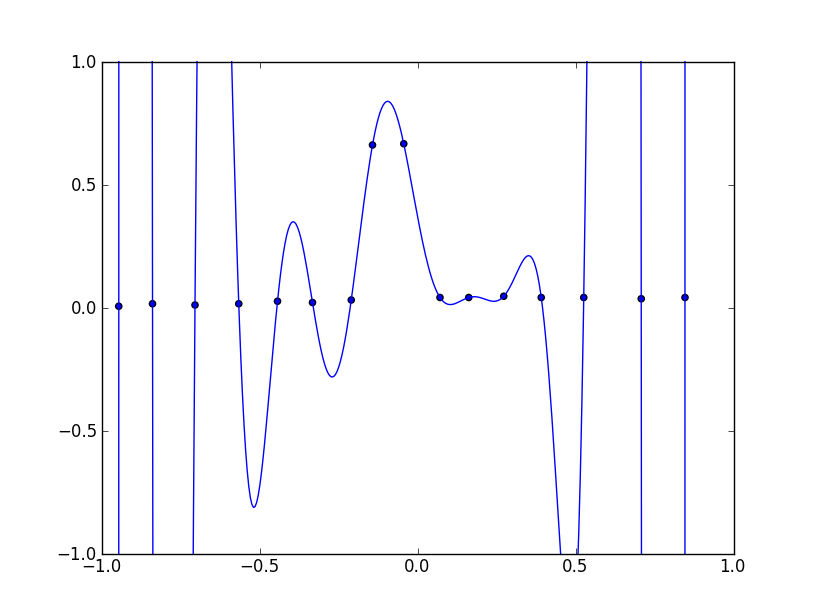
\includegraphics[width=\textwidth]{bad_interpolation2}

There is clearly a need for a more stable curve that we can manipulate easily. 
This is why B\'{e}zier curves were invented. 
The following is a geometric way of tracing out a B\'{e}zier curve for an ordered set of $n$ points. 
These are called control points. 
We would like to define a smooth curve from the first point to the last point which can be manipulated according to the position of the other points. 
We will parameterize this curve between the first and last point with respect to $t$, letting $t$ go from $0$ to $1$. 
To evaluate the curve at a given $t=T_0$ do the following:
\begin{itemize}

\item

Parameterize the lines between each of the points letting $t$ go from $0$ to $1$. 
For the points $P_{n}$ and $P_{n+1}$ this parameterization is $P_{n} (1-t) + P_{n+1} t$.

\item

Evaluate each of these parameterizations at $T_0$. 
Note that this gives $n-1$ new points.

\item

Repeat this process on the new lists until only one point is left. 
This is the value of the B\'{e}zier curve for these control points at the parameter $T_0$.

\end{itemize}

This is what is known as De Casteljau's Algorithm. 
It can be illustrated as follows:

The following are illustrations of De Casteljau's Algorithm for $4$ points at $t= 0$, $.25$, $.5$, $.75$, and $1$ respectively.

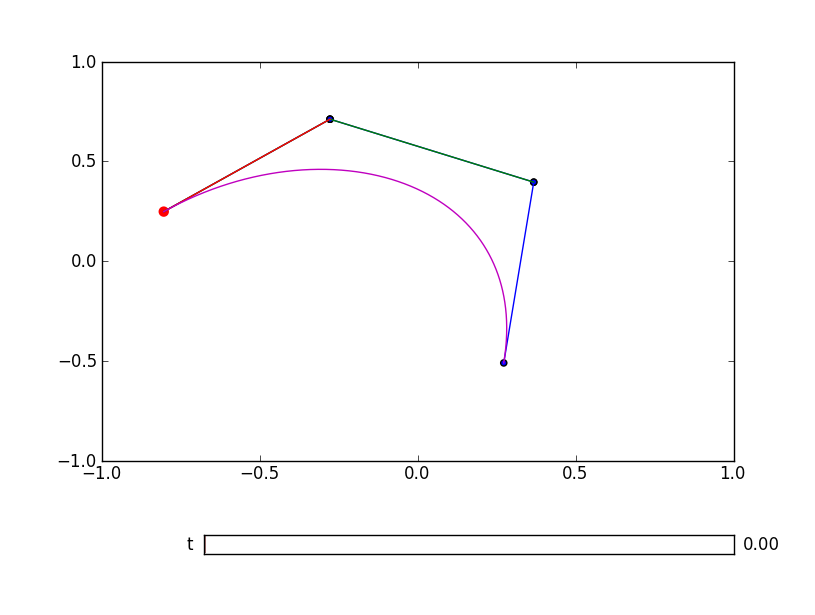
\includegraphics[width=\textwidth]{decasteljau_1}

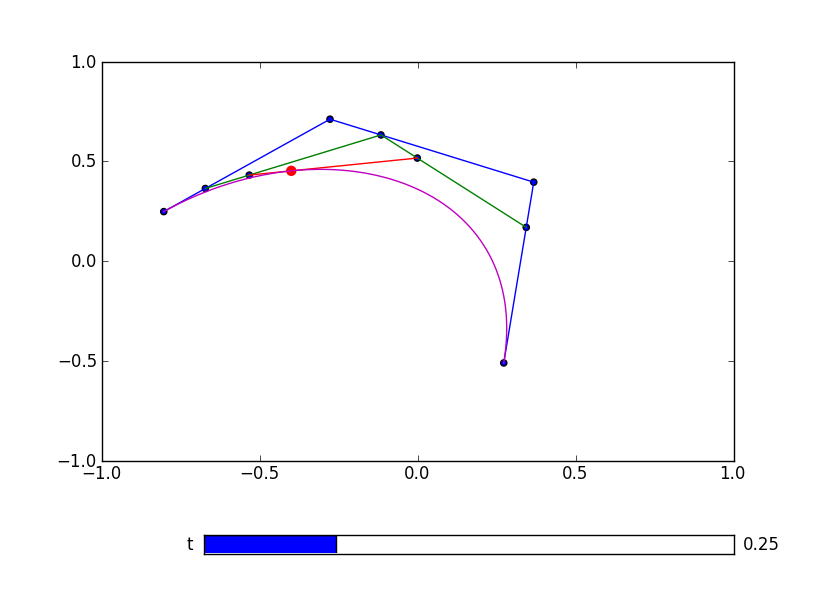
\includegraphics[width=\textwidth]{decasteljau_2}

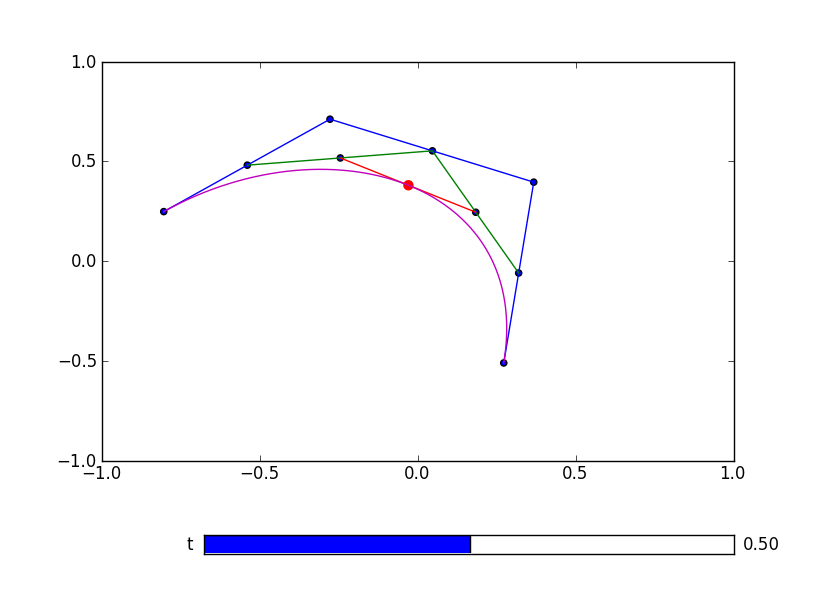
\includegraphics[width=\textwidth]{decasteljau_3}

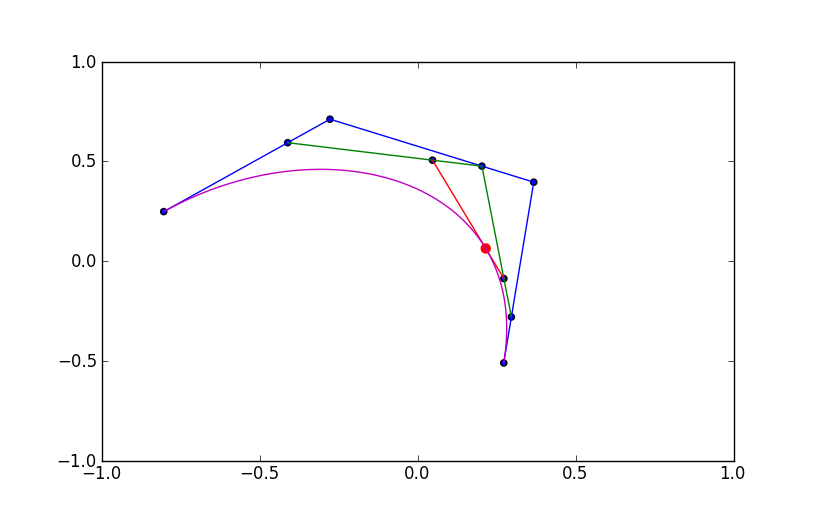
\includegraphics[width=\textwidth]{decasteljau_4}

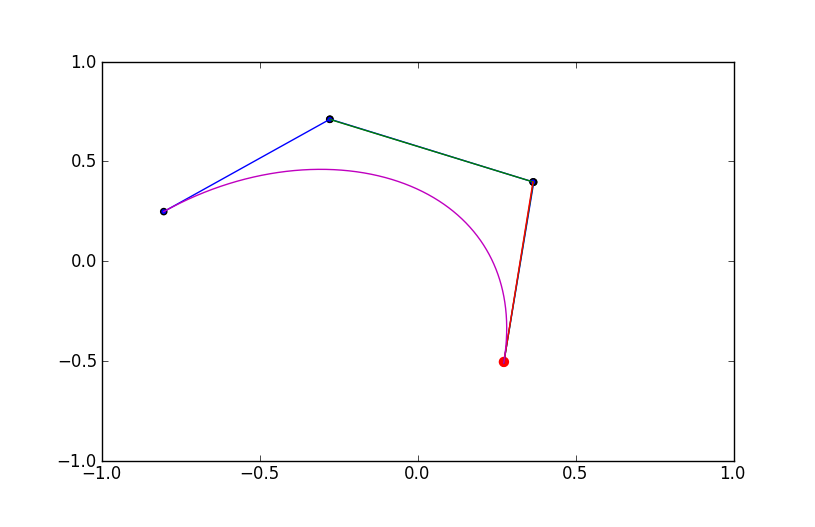
\includegraphics[width=\textwidth]{decasteljau_5} 

This algorithm is also usable for large numbers of points, though evaluation time increases rapidly.

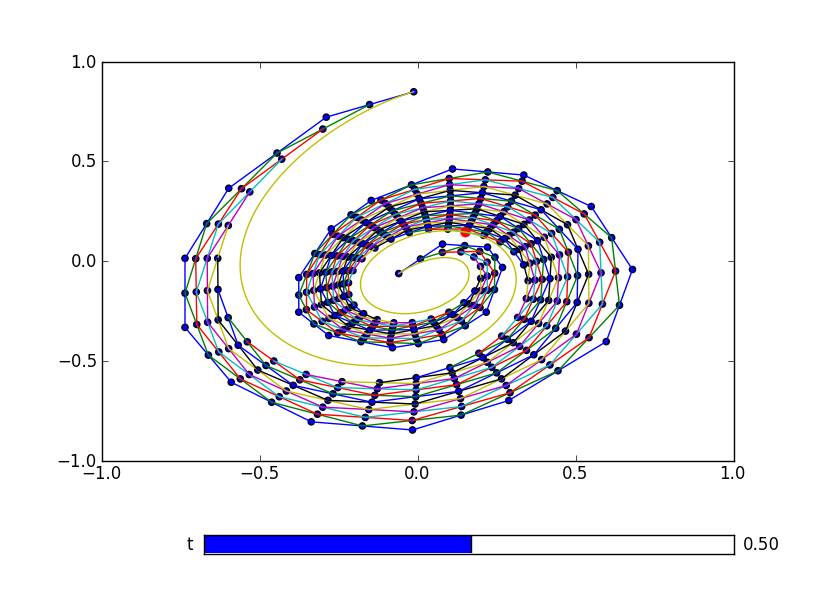
\includegraphics[width=\textwidth]{decasteljau_6}

\begin{problem}
Implement De Casteljau's algorithm.
\end{problem}

\begin{problem}
Use a slider bar to interactively show how the algorithm works. 
Use Matplotlib's \li{ginput} function to get the control points for the graph.
\end{problem}

It is important to note that these curves are only dependent upon the points themselves and not on the coordinate system with which we are viewing them. 
Since a B\'{e}zier curve is defined only by its control points, it is much easier to rotate it without changing its shape.

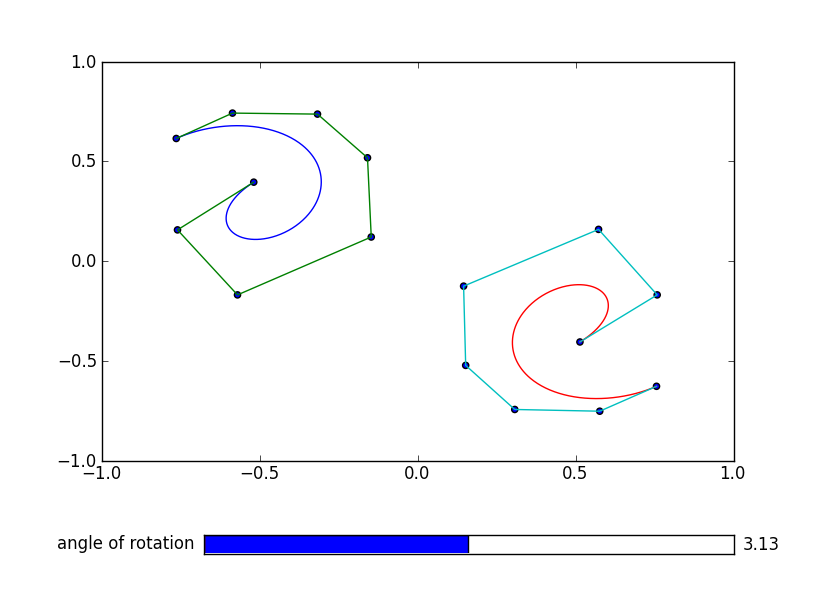
\includegraphics[width=\textwidth]{bezier_rotation}

There is a way of generating these functions explicitly. 
It is by writing the parameters of $x$ and $y$ as sums of Bernstein polynomials in $t$. 
The $k$'th Bernstein polynomial of order $n$ is written as 

$$\theta_{i,n}=\left( \begin{smallmatrix} n\\ i \end{smallmatrix} \right) (1-t)^{n-i} t^i$$

where $\left( \begin{smallmatrix} n\\ i \end{smallmatrix} \right) = \frac{n!}{i!(n-i)!}$, i.e. the binomial coefficients.

The B\'{e}zier curve for a given set of control points (also called the control polygon) is given by the formula:

$$\gamma (t) = \sum_{i=0}^n P_i \theta_{i,n} (t)$$ 

where $P_i$ is the i'th point of the control polygon.

These functions are convenient for quick evaluation of low order B\'{e}zier curves, but they are not stable for high numbers of points. 
This is because the coefficients $\left( \begin{smallmatrix} n\\ i \end{smallmatrix} \right)$ grow very rapidly for large $n$. 
For example, $\left( \begin{smallmatrix} 40\\ 20 \end{smallmatrix} \right)=137846528820$. 
The errors that can come from having these large coefficents used in each of these polynomials are not troublesome at for low degree polynomials, but they quickly become a concern for larger ones. 

\begin{problem}
Write a python function which, given the control polygon returns functions for the parameterizations of $x$ and $y$. 
You may want to use scipy polynomial objects to do this.
\end{problem}

\begin{problem}
Plot a B\'{e}zier curve with 30 randomly generated control points using De Casteljau's Algorithm. 
Try doing it with Bernstein polynomials. 
What do you observe? 
How many control points can you use before the Bernstein polynomial approach breaks down?
\end{problem}

\begin{problem}
Compare computation time for computing different orders of B\'{e}zier curves using both methods. 
For different orders of B\'{e}zier curves, test running a single point through the algorithm and running a large number of points through the algorithm. 
What do you observe?
\end{problem}

\begin{problem}
Use your implementation of De Casteljau's algorithm to make a $20\times 20$ grid of B\'{e}zier curves representing the surface $sin(xy)$ on $[-\pi,\pi]\times [-pi,\pi]$.
Use the points where the gridlines intersect as the control points for each curve. 
What do you observe?
\end{problem}
